\begin{center}
	\vspace{1em}
    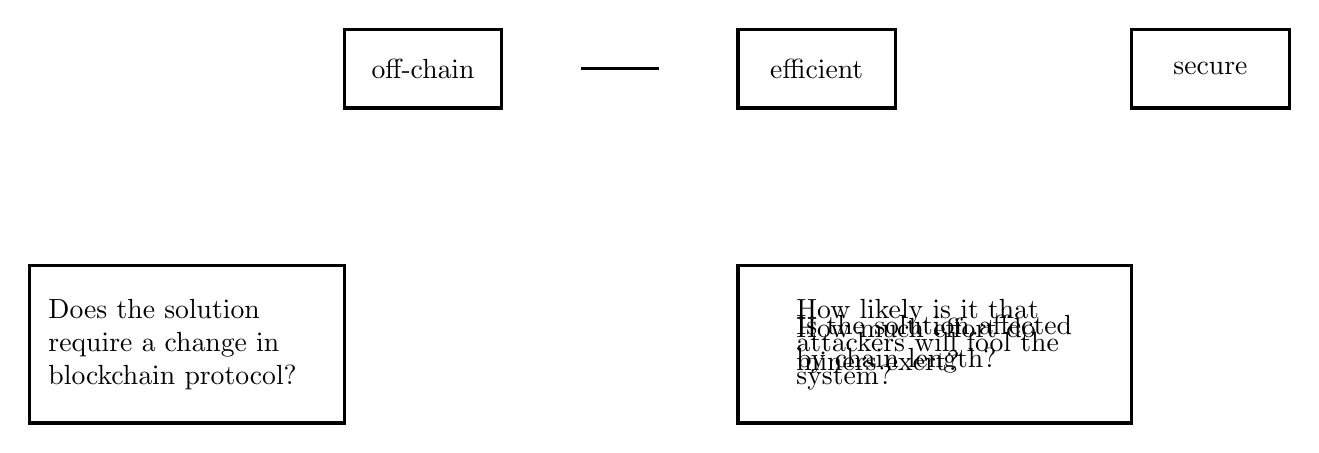
\begin{tikzpicture}
    % GQM hierarchy

    % goals
    \draw [very thick] (0,0) rectangle (2,-1) node[midway] {off-chain};
    \draw [very thick] (5,0) rectangle (7,-1) node[midway] {efficient};
    \draw [very thick] (10,0) rectangle (12,-1) node[midway] {secure};

    % questions
    \draw [very thick] (-4,-3) rectangle (0,-5) node[midway,text width=100] {{\singlespacing Does the solution require a change in blockchain protocol?}};
    \draw [very thick] (5,-3) rectangle (10,-5) node[midway,text width=100] {Is the solution affected by chain length?};
    \draw [very thick] (5,-3) rectangle (10,-5) node[midway,text width=100] {How much effort do miners exert?};
    \draw [very thick] (5,-3) rectangle (10,-5) node[midway,text width=100] {How likely is it that attackers will fool the system?};

    % lines (length 0.75)
    \draw [very thick] (3,-0.5) -- (4,-0.5);

    \end{tikzpicture}
    \captionof{figure}{Goal Question Metric hierarchy \label{fig:gqm}}
\end{center}
